\section{Results and Discussion}
Let's now demonstrate some of this functionality.
%
    \subsection{Figure Referencing}
%
With the compilation of the supporting information happening first, and the definition of a special supporting figure environment, we can very easily reference these figures in our main text.
Supporting Figure S\ref{sfig:example}.
We can also reference subfigures in our supporting figures.
Supporting Figure S\ref{sfig:sub-example1}.

We can also put some subfigures in our main text to be referenced in our response to reviewers:
\begin{figure}[H]
    \centering
    \begin{subfigure}{0.45\textwidth}
        \centering
        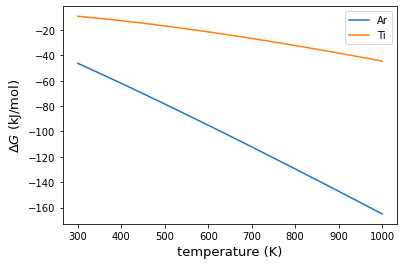
\includegraphics[width=\textwidth,keepaspectratio]{figures/DeltaG.png}
        \caption{}
        \label{fig:example1}
    \end{subfigure}
    \begin{subfigure}{0.45\textwidth}
        \centering
        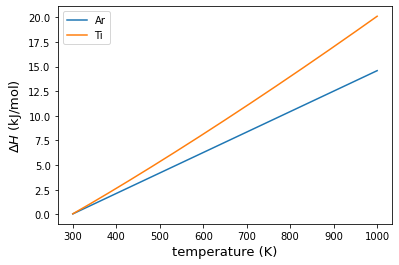
\includegraphics[width=\textwidth,keepaspectratio]{figures/DeltaH.png}
        \caption{}
        \label{fig:example2}
    \end{subfigure}
    \caption{
    (\subref{fig:example1}) basic demonstration of the subref command for a subfigure.
    (\subref{fig:example2}) The other subfigure
    }
    \label{fig:example-main}
\end{figure}
The subref command allows you to extract just the alphabetical label for the figure, while the ref command will extract the full reference.
For example, Figure \ref{fig:example1} (ref) or Figure part \subref{fig:example1} (subref).
This only works if the correct labels are attached.
%
    \subsection{Line and Page Numbers}
%
Line and page numbers are extremely useful when responding to reviewers.
As such, it's quite convenient to be able to label and reference changes between the two documents.
This line contains a label,\label{point:1} and a linelabel,\linelabel{line:1} which will allow me to reference it in the response to reviewers.
%
    \subsection{Word Counts}
%
Word counts can be done with great accuracy using \verb|texcount| which is a command line tool installed with most LaTeX distributions.
It is possible to count multiple files at once, and it provides detailed statistics.
\begin{center}
    \verb|texcount 1_introduction.tex 2_results.tex|
\end{center}
%
    \subsection{Track Changes}
%
It is possible to obtain a ``marked up'' version of your manuscript by using the command line tool \verb|latexdiff|.
This tool takes two .tex files as inputs, and outputs a .tex file which will compile to an annotated track changes version.
\begin{center}
    \verb|latexdiff oldfile.tex currentfile.tex > markup.tex|
\end{center}